\chapter{Rank Reversal}
\label{chap:rank_reversal}

The so called rank reversal phenomenon in a multi-criteria decision aid context is a phenomenon initially highlighted by Belton and Gear in 1983 \cite{belton1983short}\cite{wang2009rank}.

There is not one unique definition of the rank reversal phenomenon but there rather exist several, which however generally share the same idea: ``the relative ordering between two alternatives depends on the presence of one or several other alternatives''. \\
Some of the definitions that can be found in the literature are that the relative position of two alternatives can be influenced by the presence of \cite{Brans2016}:
\begin{itemize}
    \item a non discriminating criterion
    \item a copy of an alternative
    \item a dominated alternative
    \item any other alternative
\end{itemize}

In the rest of this work, unless stated otherwise, we will say that there is a ``rank reversal occurrence'' when the relative ordering between two alternatives is affected by the presence or absence of any third alternative.

This phenomenon can lead to some undesirable consequences. One of these obvious undesirable consequence is highlighted in the following example. \\
Suppose that a municipal administration of a city considers that it is necessary to build a new sports stadium. This could be due to the fact that the existing one is becoming too old or because its capacity is no longer sufficient to host enough supporters.
The municipal administration would therefore organise a competition where architects and entrepreneurs would propose their projects.
The administration could decide to rank all these projects using a multi-criteria decision aid method according to criteria such as the estimated price of the project, the estimated duration of the works, the capacity of the stadium, the capacity of its parking, etc.
The project arriving in first position of the ranking would be selected and built.\\
In such a situation, the possibility of a rank reversal between the first two alternatives would have important consequences as it would influence which stadium would be built, and which group of people would have the right to build it.
There does not seem to be any rational reason why the order of the two first projects should be influenced by the presence of other projects and therefore these kind of rank reversals should be avoided.

In similar situations, it could also be argumented that the multi-criteria decision aid methods which suffers from rank reversal occurrences are vulnerable to ranking manipulations by artificially adding (or removing) some alternatives.

W. De Keyser and P. Peeters \cite{de1996note} were the first to point out that the \textsc{promethee} methods suffer from rank reversal occurrences.

Before going into the specific details of the rank reversal phenomenon in \textsc{promethee}, some characteristics of more general methods based on pairwise comparisons will be given.

\section{Transitivity of preferences and pairwise \\ comparisons}
Some important facts have been highlighted by Mareschal et al. \cite{mareschal2008rank} concerning methods based on the pairwise comparisons of the alternatives.

These facts will be resumed in the rest of this section. First, the notion of \textit{consistent ranking methods based on pairwise comparison} will be defined.
Then, few words will be said about the transitivity of the preferences and finally, it will be shown that consistent ranking methods based on pairwise comparisons with nontransitive preferences matrices suffer from the rank reversal phenomenon \cite{mareschal2008rank}.


\subsection{Ranking methods based on pairwise comparisons}
\label{sec:RBPC}
Let us again consider a multi-criteria decision problem consisting in the ranking of the alternatives from a finite set $A$ of $n$ alternatives which must maximise $k$ evaluation functions.\\
\newpage
If the multi-criteria decision aid method is based on:
\begin{enumerate}
    \item the computation of an $n \times n$ pairwise preferences matrix \textit{Pref} whose elements \textit{pref}$_{ij}$ are global preference indices of the alternative $a_i$ over $a_j$
    \item the exploitation of this matrix to obtain a complete preorder
\end{enumerate}
then it is said to be a \textit{ranking method based on pairwise comparisons} (RBPC) \cite{mareschal2008rank}.

The \textsc{promethee} methods are examples of such methods where the $n \times n$ preferences matrix $\Pi$ consist in the $n \times n$ evaluations of $\pi(a_i, a_j)$ for all $a_i, a_j$ in $A$.

Furthermore, a ranking method based on pairwise comparisons is said to be \textit{consistent} if the ordering obtained with its application on a set of two alternatives is consistent with the $2 \times 2$ preferences matrix.\\
This means that if a consistent ranking method based on pairwise comparisons is applied on a set of two alternatives $a_i$ and $a_j$, with $a_i$ pairwise preferred over $a_j$ (\textit{pref}$_{ij} > $\textit{pref}$_{ji}$) then $a_i$ should be ranked before $a_j$ \cite{mareschal2008rank}.
This property seems rather intuitive and necessary for any ranking method based on pairwise comparisons.

By remembering how the outranking flow is computed in \textsc{promethee} (section \ref{sec:outranking_flow}), one can easily see that it will be consistent with any $2\times 2$ preferences matrix $\Pi$. 
This means that \textsc{promethee} is a consistent ranking method based on pairwise comparisons.
It should however be noted that the ranking obtained with a larger set of alternatives will not necessarily respect all the pairwise preferences anymore. 

As already announced, such methods with nontransitive preferences matrix are susceptible to suffer from the rank reversal phenomenon.
One could therefore wonder why these preferences matrix could be nontransitive.
Some insights into the transitive nature of the preferences will therefore be given in the next section.
% \subsection{Rank reversal in consistent RBPC with intransitive preferences matrix}
% If a multi-criteria method is based on pairwise comparisons, is consistent and is applied on a preferences matrix that is not transitive, then the rank reversals are unavoidable
% One could object that the preferences matrix should be transitive.
%

\subsection{Transitivity of the preferences}
In a mono-criterion context, with a criterion $f(.)$ which must be maximized, the preference relation $P$ of the natural dominance relation is trivially transitive:
\begin{equation}
    \forall a_i, a_j, a_k \in A: \left \{
        \begin{array}{l}
            a_iPa_j \Rightarrow f(a_i) > f(a_j) \\
            a_jPa_k \Rightarrow f(a_j) > f(a_k)
        \end{array} \right .
        \Rightarrow f(a_i) > f(a_k) \Rightarrow a_iPa_k
    \label{eqn:transitivity_preference_monocriterion}
\end{equation}

In a similar way, one could see that the indifference relation is also transitive.

A slightly more elaborated dominance relation can be defined by introducing an indifference threshold $q$:

\begin{equation}
    \forall a_i, a_j \in A: \left\{
        \begin{array}[]{l c c c c}
            f(a_i)  >  f(a_j) + q           &\Leftrightarrow & a_iPa_j \\
            \mid f(a_i) - f(a_j) \mid  \leq  q  &\Leftrightarrow & a_iIa_j \\
            f(a_i)  <  f(a_j)  -q             &\Leftrightarrow & a_jPa_i \\
        \end{array}
        \right .
    \label{eq:dominance_relation_monocriterion_ind_threshold}
\end{equation}

This dominance relation defines a \textit{semiorder} \cite{Vin92}. The preference relation $P$ is still transitive but the indifference $I$ relation is not transitive anymore.
\begin{equation}
    \begin{split}
    \forall a_i, a_j, a_k \in A: \left \{
        \begin{array}{l}
            a_iPa_j \Rightarrow f(a_i) > f(a_j)+q \\
            a_jPa_k \Rightarrow f(a_j) > f(a_k)+q
        \end{array} \right . \\
        \Rightarrow f(a_i) > f(a_k)+q \Rightarrow a_iPa_k
    \end{split}
    \label{eqn:transitivity_preference_monocriterion_indiff_threshold}
\end{equation}
The semiorder dominance structure has been introduced by Luce in \cite{Luce1956} as a way to represent the human preference model (preference and indifference) without relying on the assumption that the indifference relation is transitive.
This hypothesis is justified between others by the fact that a human being cannot discriminate between two evaluations if these are to close one to another. \\
Luce gives the example of 401 numbered cups of coffee where each cup of coffee $i$ would contain $\big( 1+ \frac{i}{100} \big) x$ grams of sugar, with $i=1\dots401$ and $x$ being the weight in grams of a cube of sugar.
When asking to someone to taste any cups $i$ and $i+1$, he will obviously not taste any difference.
On the other hand, when asking to someone to taste the first and the last cup, it is highly probable that he will taste a difference \cite{Luce1956}.

Tversky goes a step further and shows that when considering a multi-criteria context, even the preference relation should not be considered as being necessarily transitive \cite{tversky1969}.
Tversky motivate his statement with the following example.

Consider a decision maker $D$ which must hire one of three possible candidates. The candidates are evaluated according to two criteria: \textit{intelligence} and \textit{experience}. The evaluations of the different candidates can be seen in Table \ref{tbl:tversky_non_transitive_preferences}.


\begin{table}[h]
\center
\begin{tabular}{ l c c c }
    \toprule
     Candidates & & Intelligence   & Experience  \\
     \cmidrule(rl){1-1}   \cmidrule{3-4}
      $x$  & & $2\varepsilon$       & $6\varepsilon$              \\
      $y$  & & $3\varepsilon$       & $4\varepsilon$            \\
      $z$  & & $4\varepsilon$       & $2\varepsilon$            \\
    \bottomrule
\end{tabular}
\caption{Evaluation table of Tversky's example \cite{tversky1969}}
\label{tbl:tversky_non_transitive_preferences}
\end{table}

The evaluations represent some dimensionless scores according to the corresponding criteria with $\varepsilon$ being a constant.

Suppose $D$ values the intelligence more than the experience.
He could therefore adopt the following strategy: 
\begin{itemize}
    \item If a candidate $c_i$ is considered by the decision maker $D$ as more intelligent than a candidate $c_j$, then candidate $c_i$ will be preferred over $c_j$.
    \item If two candidates $c_i$ and $c_j$ are both considered by $D$ as being equally intelligent, then the one with the most experience will be preferred.
\end{itemize}

Now suppose also that $D$ does not find that a difference of score smaller or equal to $\varepsilon$ for the intelligence criterion is enough to be significative (this can be due to the fact that the tests are not precise enough, or simply because $D$ does not care about too small differences).
The ranking of the candidates, based on the intelligence criterion only, will therefore lead to a semiorder structure (as the ones introduced by Luce).\\

This has for consequence that the candidate $y$ is considered by $D$ as being equally intelligent to both the two other candidates, but candidates $x$ and $z$ are not considered as equally intelligent ($z$ being considered more intelligent than $x$).
Since $y$ is considered as equally intelligent as $x$ and $z$, the preference between these pairs will depend on the experience of the candidates.

By defining ($I_{int}, P_{int}$) and ($I_{exp}, P_{exp}$) the indifference and preference relations respectively on the intelligence and experience criterion only, the following preference relations are obtained:
\begin{equation}
    \begin{split}
     \left \{
        \begin{array}{l l}
            yI_{int}z \ \land \ yP_{exp}z \ & \Rightarrow yPz \\
            yI_{int}x \ \land \ xP_{exp}y \ & \Rightarrow xPy \\
            zP_{int}x                 & \Rightarrow zPx
        \end{array} \right . \\
    \end{split}
    \label{eqn:candidates_nontransitive_dominance_rel}
\end{equation}

These considerations will lead to the preferences matrix represented in Figure \ref{fig:untransitive_matrix}.

\begin{figure}[h]
\begin{minipage}{.5\textwidth}
    \begin{equation*}
        P   = \bordermatrix{~ & x    & y    & z   \cr
                            x & 0    & 1    & 0   \cr
                            y & 0    & 0    & 1   \cr
                            z & 1    & 0    & 0   \cr}
        \label{eq:transitive_pref_example}
    \end{equation*}
\end{minipage}
\begin{minipage}{.5\textwidth}
    \begin{center}
     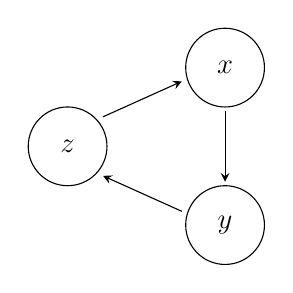
\begin{tikzpicture}[scale=0.5, transform shape]
        % before suppression of alternative
        \draw (4,-2) circle (1) ;
        \draw (4,-2) node{\huge{$y$}};
        \draw (4,2) circle (1) ;
        \draw (4,2) node{\huge{$x$}};
        \draw (0,0) circle (1) ;
        \draw (0,0) node{\huge{$z$}};
        \draw [>=stealth,->] (0.90,0.75) -- (2.90,1.65);
        \draw [>=stealth,->] (2.90,-1.65)-- (0.90,-0.75) ;
        \draw [>=stealth,->] (4,0.9)    -- (4,-0.9) ;
        %\draw [>=stealth,->] (1,2.25) -- (3,3.75);
        % after deletion of a2
        \end{tikzpicture}
   \end{center}
\end{minipage}%
\caption{Example of non transitive preferences matrix and its graphical representation} \label{fig:untransitive_matrix}
\end{figure}

Unlike with the pairwise preferences matrices $\Pi$ of the \textsc{promethee} methods whose elements are valued between $0$ and $1$ and represent the strength with which an element is pairwise preferred over another, this matrix is binary and indicates if an alternative is preferred over another, without giving any indication about the strength of the preference.

It can be seen from this example, that the pairwise preferences of a decision maker which seems to use only reasonable assumptions can be nontransitive.

It will now be shown that any ranking method based on pairwise comparisons which is consistent and uses a nontransitive preferences matrix must suffer from the rank reversal phenomenon.

\subsection{Rank reversal occurrences in consistent RBPC with nontransitive preferences}

To demonstrate that rank reversal occurrences are unavoidable in such conditions, we will consider the problem of having to rank the three candidates presented in the previous section. \\
The considered ranking method will therefore have to aggregate the nontransitive preferences in one global ranking, as shown in Figure \ref{fig:aggregating_nontrans}.
\vskip 0.15cm

\begin{figure}[h]
    \centering
    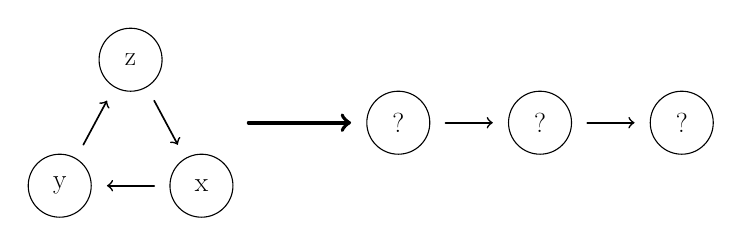
\begin{tikzpicture}[scale=0.4, transform shape, line cap=round,x=1.0cm,y=1.0cm]
        %\clip(-7.7,-4.66543927909192) rectangle (6.858736141587812,4.56639472090804);
        \draw(-1.75,-2.) circle (1.cm) ;  %x
        \draw(-6.25,-2.) circle (1.cm);   %y
        \draw(-4.,2.) circle (1.cm);    %z
        \draw [->,line width=0.6pt] (-5.5,-0.70) -- (-4.75,0.7);     % ab
        \draw [->,line width=0.6pt] (-3.25,0.7) -- (-2.50,-0.700);        % bc
        \draw [->,line width=0.6pt] (-3.25, -2) -- (-4.75, -2);
        \draw(9.,0) circle (1.cm)   ;
        \draw(4.5,0.) circle (1.cm) ;
        \draw(13.5,0.) circle (1.cm);
        \draw [->,line width=0.6pt] (10.5,-0.) -- (12,0.); %23
        \draw [->,line width=0.6pt] (6.,0) -- (7.5,0.);         %12
        \draw [->,line width=1.4pt] (-0.25,0.) -- (3.,0.);
        \draw (9.,0) node {\Huge ?};  %2
        \draw (4.5,0) node {\Huge ?};    %1
        \draw (13.5,0.) node {\Huge ?}; %3
        \draw (-6.25,-2.) node[] {\Huge y};
        \draw (-4.,2.) node[] {\Huge z};
        \draw (-1.75,-2.) node[] {\Huge x};
    \end{tikzpicture}
    \caption{Aggregating non transitive preferences in a ranking} \label{fig:aggregating_nontrans}
\end{figure}

Since the method is considered to be consistent by hypothesis, if one alternative is removed, the ranking obtained by applying the method on the remaining alternatives must respect the pairwise preferences of these alternatives (since the method is applied on only two alternatives).
These conditions are shown in the Figure \ref{fig:consistent_rankings}.

\vskip 0.15cm
\begin{figure}[h]
    \begin{minipage}{0.3\textwidth}
        \centering
        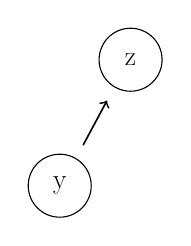
\begin{tikzpicture}[scale=0.4, transform shape, line cap=round,x=1.0cm,y=1.0cm]
            \draw(-6.25,-2.) circle (1.cm);   %a
            \draw(-4.,2.) circle (1.cm);    %b
            \draw [->,line width=0.6pt] (-5.5,-0.70) -- (-4.75,0.7);     % ab
            \draw (-6.25,-2.) node[] {\Huge y};
            \draw (-4.,2.) node[] {\Huge z};
        \end{tikzpicture}
    \end{minipage}
    \begin{minipage}{0.3\textwidth}
        \centering
            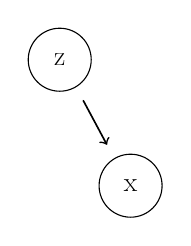
\begin{tikzpicture}[scale=0.4, transform shape, line cap=round,x=1.0cm,y=1.0cm]
            %\clip(-7.7,-4.66543927909192) rectangle (6.858736141587812,4.56639472090804);
            \draw(-1.75,-2.) circle (1.cm);  %c
            \draw(-4.,2.) circle (1.cm);    %b
            \draw [->,line width=0.6pt] (-3.25,0.7) -- (-2.50,-0.700);        % bc
            \draw (-4.,2.) node[] {\Huge z};
            \draw (-1.75,-2.) node[] {\Huge x};
            \end{tikzpicture}
    \end{minipage}
    \begin{minipage}{0.3\textwidth}
        \centering
            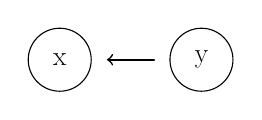
\begin{tikzpicture}[scale=0.4, transform shape, line cap=round,x=1.0cm,y=1.0cm]
            %\clip(-7.7,-4.66543927909192) rectangle (6.858736141587812,4.56639472090804);
            \draw(-1.75,-2.) circle (1.cm);  %c
            \draw(-6.25,-2.) circle (1.cm);   %a
            \draw [->,line width=0.6pt] (-3.25, -2) -- (-4.75, -2);
            \draw (-6.25,-2.) node[] {\Huge x};
            \draw (-1.75,-2.) node[] {\Huge y};
            \end{tikzpicture}
    \end{minipage}
    \caption{Consistent rankings when only two candidates are considered} \label{fig:consistent_rankings}
\end{figure}

It should be quite obvious that it is not possible to find any complete ranking that satisfies these three conditions.
Therefore, whatever the ranking is, it will lead to some rank reversal occurrence when one of the alternatives is removed.\\
The reasoning here above has been done for three alternatives but it remains valid for any set of alternatives where the pairwise preferences between these alternatives form a cycle (such as in figure \ref{fig:untransitive_matrix}).
We can therefore conclude that the rankings obtained with \textsc{promethee} on a set of alternatives, from which a subset have nontransitive pairwise preferences, will inevitably suffer from rank reversal occurrences.

However, this is not the only characterization that can be done concerning the possibility of occurrence of rank reversals in the \textsc{promethee} methods.
The next section will address the possibility of rank reversal occurrences between alternatives dominating each other and the impact of the differences of net flows of two alternatives on their possibility to reverse their ranks. % between alternatives whose net flows are ``distant enough''.


\section{Some results about the rank reversal \\ phenomenon in the \textsc{promethee} methods}

\subsection{Respect of the natural dominance relation} \label{sec:pii_respect_dominance}

An alternative which is at least as good as another alternative on all the criteria and strictly better on at least one criteria is said to dominate this other alternative (see section \ref{sec:multi_criteria_dominance_rel}).
There is obviously no reason why an alternative which is dominated by another should be ranked before this other which would be a violation of the natural dominance relation.
It is therefore reasonable to hope that any ranking method will respect it.\\
This also means that there should not be any strict rank reversal between dominated and dominant alternatives (the dominated alternatives could however become indifferent to the dominant ones under some particular circumstances).

It will be shown here under that the \textsc{promethee} methods respect the dominance relation \cite{DecisionEng} and do not suffer from these kind of rank reversals.

% Assume a finite set $A$ of $n$ alternatives that must maximise a set of $k$ evaluations functions ($f_c(.)$). 
It will be shown that if alternative $a_i$ is dominating alternative $a_j$, then its netflow can not be lower that the one of $a_j$:

\begin{equation}
    \begin{split}
     \left \{
        \begin{array}{l l}
            \forall c=1,\dots, k \ :\qquad & f_c(a_i) \ge f_c(a_j) \\
            \exists h \in \{1,\dots,k\}: \qquad & f_c(a_i) > f_c(a_j)
        \end{array} \right .
        \Rightarrow \phi(a_i) \ge \phi(a_j)
    \end{split}
    \label{eqn:ai_dominates_aj}
\end{equation}

Since $a_i$ is dominating $a_j$, and the preference functions $P_c$ are nondecreasing, we can see that $\pi(a_i,b) \ge \pi(a_j,b)$ for any $b$ in $A$:
\begin{align}
    \begin{split}
        \pi(a_i, b) = \sum\limits^k_{c=1} w_c \cdot P_c(a_i,b)
                    \ge \sum\limits^k_{c=1} w_c \cdot P_c(a_j,b)
                    = \pi(a_j, b)
    \end{split}
    \label{eqn:pi_aib_ge_pi_ajb}
\end{align}

A similar reasoning can be applied to see that $\pi(b,a_i) \le \pi(b, a_j)$.

Therefore we can conclude that:
\begin{align}
    \begin{split}
    \phi(a_i) & = \phi^+(a_i) - \phi^-(a_i) \\
              & = \frac{1}{n-1}\sum\limits_{b\in A} \pi(a_i,b) - \frac{1}{n-1}\sum\limits_{b\in A} \pi(b, a_i)\\
              & \ge \frac{1}{n-1}\sum\limits_{b\in A} \pi(a_j,b) - \frac{1}{n-1}\sum\limits_{b\in A} \pi(b, a_j) \\
              & \ge \phi(a_j)
    \end{split}
    \label{eqn:dominance_demo_phi_ai}
\end{align}

Showing that the dominance relation is respected.

\subsection{Rank reversal and net flow differences}

Having alternatives dominating each other is not the only situation under which rank reversal cannot occur in the \textsc{promethee} methods.
Indeed, rank reversal can occur only between alternatives whose net flows difference is lower than a given limit.

Here under, an initial bound on the net flow difference between two alternatives will be shown under which rank reversal cannot occur when one alternative is removed in \textsc{promethee ii} \cite{DecisionEng}.

% Suppose a set of alternatives $A$ from which an alternative $x$ is removed. The resulting set will be noted $A^{\prime}$. The net flow of an alternative $a_i$ in the new set is given by:
Suppose that alternative $x$ is removed from the set of alternatives $A$. The resulting set will be noted $A^{\prime}$. The net flow of an alternative $a_i$ in the new set is given by:
\begin{align}
    \begin{split}
        \phi^{\prime}(a_i) & =
            \frac{1}{n-2}\sum\limits_{b\in A^{\prime}} (\pi(a_i,b) - \pi(b, a_i)) \\
            & = \frac{1}{n-2}\sum\limits_{b\in A} (\pi(a_i,b) - \pi(b, a_i)) - \frac{1}{n-2}(\pi(a_i,x) - \pi(x,a_i))\\
            &= \frac{n-1}{n-2}\phi(a_i) - \frac{1}{n-2}(\pi(a_i,x) - \pi(x,a_i))\\
    \end{split}
    \label{eqn:phi_a_prime_using_phi_a}
\end{align}

Using the same reasoning for an alternative $a_j$, we can express the net flow difference between the two alternatives in the set $A^{\prime}$ according to their net flow difference in $A$:
\begin{align}
    \begin{split}
        \phi^{\prime}(a_i) - \phi^{\prime}(a_j)
             = & \frac{n-1}{n-2}(\phi(a_i) - \phi(a_j)) \\
                & - \frac{1}{n-2}(\pi(a_i,x) - \pi(x,a_i) - \pi(a_j,x) + \pi(x, a_j))\\
    \end{split}
    \label{eqn_phi_diff_prime_using_phi_diff}
\end{align}

If we suppose that $a_i$ was initially ranked before $a_j$ ($\phi(a_i) - \phi(a_j)> 0$), there will be no rank reversal ($\phi^{\prime}(a_i) - \phi^{\prime}(a_j)> 0$) only if:
\begin{align}
        (n-1)(\phi(a_i) - \phi(a_j) > (\pi(a_i,x) - \pi(x,a_i) - \pi(a_j,x) + \pi(x, a_j))
    \label{eqn:no_rr_phi_condition_using_x}
\end{align}

By remembering that $\pi(a_{\alpha}, a_{\beta})$ can only take values between zero and one (see equation \ref{eq:pi_bounds} in section \ref{subsec:global_pref_index}) we can conclude that there cannot be any rank reversal between $a_i$ and $a_j$ when an alternative is removed if their net flow difference is greater than:
\begin{align}
    \begin{split}
        (n-1)(\phi(a_i) - \phi(a_j) & > (1 - 0 - 0 + 1) \\
        \phi(a_i) - \phi(a_j) & > \frac{2}{n-1}
    \end{split}
    \label{eqn:no_rr_condition}
\end{align}

This bound, which is only valid when one alternative is removed, can however be generalized to the cases where $N$ alternatives are removed:
\begin{align}
    \phi(a_i) - \phi(a_j) > \frac{2N}{n-1}
    \label{eqn:no_rr_generalization}
\end{align}

However, this first bound is quite weak and not really often applicable.
A reinforcement of this bound has been given in \cite{Verly2013} where it is shown that the removal of one alternative cannot cause any rank reversal between alternatives which's net flow difference is greater than:
\begin{align}
    \phi(a_i) - \phi(a_j) > \frac{2}{n-1}\cdot W_{ij}
    \label{eqn:rr_bound_verly}
\end{align}

where:
\begin{align}
    W_{ij} = \sum\limits_{c=1, f_c(a_i) \ge f_c(a_j)}^k w_c
    \label{eqn:Wij}
\end{align}
represents the total weight of the coalition of criteria where $a_i$ is as least as good as $a_j$ \cite{Verly2013}.

\section{Comments about the rank reversal phenomenon and conclusion}

As it has been seen, the rank reversal problem is far from being a trivial one.
There seems to be situations where the rank reversal phenomenon could be seen as reasonable (with nontransitive preferences) but there are also cases where it should be avoided (such as in the example of the sport stadium). 

It should also be noted that this phenomenon is not restricted to the area of multi-criteria decision aid.
Indeed, it had already been highlighted earlier in social choice theory, and more particularly in Kenneth Arrow's famous impossibility theorem \cite{arrow1950difficulty} and its condition of \textit{Independence of irrelevant alternatives}.

The problematic of rank reversal in the multi-criteria decision aid domain has already been addressed and is still addressed by numerous authors (some of them have already been mentioned in this chapter) and it is important to point out that the issue of the legitimacy of this phenomenon has not been settled yet.

% The rest of this work is not aimed at answering to the question of the legitimacy of this phenomenon.
The rest of this work is not aimed at answering this question. 
It rather starts from the ascertainment that rank reversals occurs in the \textsc{promethee} methods, and proposes an investigation of two approaches aimed at reducing or suppressing them.

The first approach is called \textsc{robust promethee} and will be described in the next chapter.
It is based on the repetition of \textsc{promethee ii} a great number of times on small subsets of alternatives chosen at random. 

The second approach is called \textsc{referenced promethee}. It is based on the application, for each of the considered alternatives, of \textsc{promethee ii} on a set constituted of this alternative and of predefined reference profiles. This method, by construction, does not suffer from rank reversals.

These two methods unfortunately do not provide solutions without any cost. The distinctive features of these methods, as well as the additional information needed from the decision maker for each of them will be detailed in their corresponding chapters.




